
\chapter{Manual de usuario e instalación}
\label{cha:manual-usuario-instalacion}

\section{Introducción}
\label{sec:intro-manual-de-usuario}

En este apéndice se va a dividir en dos secciones diferenciadas donde se va a explicar como instalar y configurar todas las herramientas necesarias para la puesta a punto del proyecto. Y por otro lado, un manual de usuario donde se va a explicar como ejecutar cada uno de los algoritmos se han utilizado en el capítulo \ref{cha:resultados}.
Cabe destacar que, tal y como se indica en el sección \ref{sec:intro-pliego} del Apéndice \ref{cha:pliego-de-condiciones}, el equipo donde se instalará todo el software descrito en este apartado para programar los distintos algoritmos, se ha optado por utilizar un sistema operativo Ubuntu 18.04.4 LTS. Por tanto, todos los comandos de instalaciones y puesta en funcionamiento están orientados a un equipo que disponga de Linux.


\section{Guía de instalación}
\label{sec:sec-guia-instalacion}

\subsection{Instalación de Git}
\label{subsec:instalacion-git}

Git se trata de una herramienta de control de versiones distribuido de código que trabaja de una manera muy rápida y potente. Tiene un sistema para trabajar mediante ramas que pueden seguir una linea de progreso diferente a la principal, de tal manera que se pueden hacer pruebas del código o que distintas personas trabajen en ramas distintas y posteriormente, cuando haya una versión final, se pueda incluir en la rama principal. Para proyectos como el presente, es necesario de tener disponible historial completo de versiones para su correcto desarrollo.

Para poder instalar Git abra el terminal y ejecute los siguientes comandos:

\vspace{0.5cm}
\begin{lstlisting}[language=iPython,caption=Instalación de Git,captionpos=b,label={lst:install-git}]
# Actualizar paquetes de los repositorios
sudo apt-get update

# Instalacion de Git con todas sus depedencias
sudo apt-get install git-all
\end{lstlisting}

\subsection{Instalación de Anaconda}
\label{subsec:instalacion-anaconda}

Anaconda se trata de la \textit{suite} más compleja para la Ciencia de Datos en R y Python, lenguajes de programación que actualmente son líderes en Machine Learning, Inteligencia Artificial y Big Data. Esta \textit{suite} gratuita y multiplataforma dispone de las \gls{ide}'s y librerías adecuadas para su manejo. Con ellos se evita tener que instalar manualmente un \gls{ide} y el lenguaje Python con sus correspondientes librerías que en ocasiones puede ser una operación tediosa y compleja.

\begin{enumerate}
    \item Accede al siguiente enlace \cite{inst-conda} disponible en la bibliografía y descargue la versión más reciente del instalador de Anaconda para Linux:
    
    \begin{figure}[ht]
    \centering
    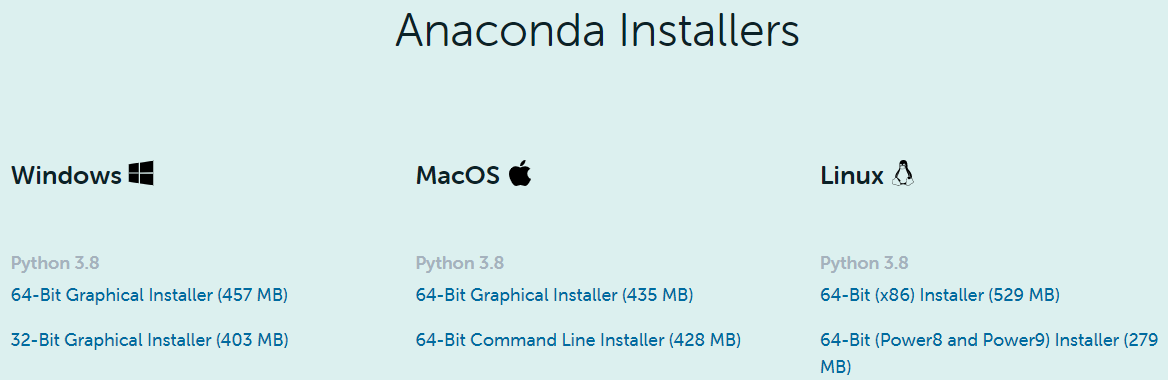
\includegraphics[width=0.8\textwidth]{img/appendix/C/anaconda-installer.png}
    \caption{\label{fig:anaconda-download}Descarga del instalador de Anaconda}
    \end{figure}

    \item Abra el terminal y acceda a la carpeta \texttt{Downloads} donde ha descargado el instalador. Es recomendable verificar la integridad del instalador mediante la suma de comprobación SHA-256:
    
    \vspace{0.5cm}
    
    % Los siguientes \begin{lstlisting}[... no están tabulados porque si no se crea una linea adicional de en las celdas
    % además de que saldría todo el código tabulado dentro de las celdas y no queda bien
    
\begin{lstlisting}[language=iPython,caption=Verificación de la integridad de la instalación de Anaconda,captionpos=b,label={lst:verificar-sha256}]
# Acceder a la carpeta Downloads del usuario
cd /home/<username>/Downloads

# Verificacion de la integridad del instalador
sha256sum Anaconda3-2020.02-Linux-x86_64.sh
\end{lstlisting}
    
    \item Ejecute la secuencias de comandos de Anaconda. Presione \texttt{yes} para aceptar los términos de la licencia. Pulse acontinuación \texttt{ENTER} cuando seleccione la ubicación de la instalación y finalmente presione \texttt{yes} para confirmar el \texttt{PATH} de Anaconda con tu \texttt{.bashrc}:
    
    \vspace{0.5cm}
    
\begin{lstlisting}[language=iPython,caption=Ejecutar el instalador de Anaconda para Linux,captionpos=b,label={lst:install-conda}]
# Ejecutar el instalador de Anaconda para Linux
bash Anaconda3-2020.02-Linux-x86_64.sh
\end{lstlisting}
    
    \item Cuando se complete la instalación cierre y abra el terminal de nuevo, o bien ejecute el siguiente comando:
    
    \vspace{0.5cm}
    
\begin{lstlisting}[language=iPython,caption=Hacer efectivo los cambios en el fichero .bashrc,captionpos=b,label={lst:source-bashrc}]
# Hacer efectivos los cambios realizados en .bashrc
source /home/<username>/.bashrc
\end{lstlisting}
\end{enumerate}

\subsection{Descarga del repositorio del proyecto}
\label{subsec:descarga-repo}

En esta subsección se indica como descargar el repositorio donde se ha programado los algoritmos de detección de objetos abandonados. Para ello se debe de seguir los comandos que se muestran a continuación:

\vspace{0.5cm}

\begin{lstlisting}[language=iPython,caption=Descarga repositorio,captionpos=b,label={lst:descarga-repo}]
# Acceder a la carpeta Documents del usuario
cd /home/<username>/Documents

# Clonar el repositorio de GitHub
git clone https://github.com/jmudy/yolov4-deepsort.git

# Acceder dentro de la carpeta clonada
cd yolov4-deepsort
\end{lstlisting}

\subsection{Crear entorno virtual con Anaconda}
\label{subsec:creacion-entorno}

Con la finalidad de evitar tediosa y larga instalación de \gls{cuda} y \gls{cudnn} y tener únicamente instaladas las librerías necesarias para que funcione el código se va a instalar un entorno virtual en Anaconda.

Desde la misma carpeta del repositorio de Github \ref{lst:descarga-repo} que se ha clonado hay dos ficheros con extensión .yml, donde viene indicadas la versión de Python que se va a necesitar, la versión de \gls{cuda} y \gls{cudnn} así como las librerías y dependencias necesarias. Para utilizar \gls{cuda} es necesario disponer de una \gls{gpu} de NVIDIA. Es muy importante verificar la capacidad de cálculo de la tarjeta gráfica NVIDIA que se emplea. En la siguiente dirección \cite{cuda-gpus} se puede comprobar la capacidad de cálculo los distintos modelos:

La capacidad de cálculo mínima para poder utilizar \gls{cuda} con al librería tensorflow-gpu es de 3.5. En función de la \gls{gpu} que dispongas, ejecute uno de los siguientes comandos para crear un entorno virtual de Anaconda con Python 3.7.0:

\vspace{0.5cm}

\begin{lstlisting}[language=iPython,caption=Creación entorno virtual en Anaconda,captionpos=b,label={lst:crear-env}]
# Si tu GPU tiene una capacidad de calculo < 3.5
conda env create -f conda-cpu.yml

# Si tu GPU tiene una capacidad de calculo >= a 3.5
conda env create -f conda-gpu.yml
\end{lstlisting}

Una vez instalado el entorno virtual se puede acceder a él ejecutando el siguiente comando:

\vspace{0.5cm}

\begin{lstlisting}[language=iPython,caption=Activar entorno virtual de Anaconda,captionpos=b,label={lst:activar-env}]
# Si instalaste el entorno con conda-cpu.yml
conda activate yolov4-cpu

# Si instalaste el entorno con conda-gpu.yml
conda activate yolov4-gpu
\end{lstlisting}

\subsection{Descargar los datasets}
\label{subsec:descarga-datasets}

Los enlaces para descargar los datasets que se han utilizado para evaluar dos distintos algoritmos a lo largo del proyecto se encuentran a continuación:

\begin{itemize}
    \item \gls{pets} dataset \url{http://www.cvg.reading.ac.uk/PETS2007/data.html} \cite{pets2007-dataset}
    \item \gls{avss} dataset \url{http://www.eecs.qmul.ac.uk/~andrea/avss2007_d.html} \cite{AVSSAB2007-dataset}
    \item \gls{gba2018} dataset \url{http://www.geintra-uah.org/datasets/gotpd1} \cite{gba-dataset}
    \item \gls{aboda} dataset \url{https://github.com/kevinlin311tw/ABODA} \cite{aboda-dataset}
    \item \gls{coco} dataset \url{https://cocodataset.org/#download} \cite{lin2015microsoft}
    \item \gls{oidv4} dataset \url{https://storage.googleapis.com/openimages/web/index.html} \cite{Kuznetsova_2020}
    
    
    
    
\end{itemize}

\section{Manual de usuario}
\label{sec:manual-usuario}

En esta parte se especifica los comandos que se deben que ejecutar para poner en funcionamiento el algoritmo de detección de objetos, el algoritmo de seguimiento o \textit{tracking} de personas y objetos y por último el algoritmo el cual determinar si un objeto ha sido abandonado o perdido.
\pendiente{Queda pendiente este apartado que podrá ser completado cuando termine de redactar los apartados de desarrollo de algoritmo de detección de objetos abandonados}

\subsection{Ejecutar algoritmo de detección de objetos YOLOv4}
\label{subsec:ejecutar-deteccion-yolov4}

\vspace{0.5cm}
\begin{lstlisting}[language=iPython,caption=Funciones de object tracking ,captionpos=b,label={lst:object-tracking}]
def init_deepsort_params():
    # Definition of the parameters
    max_cosine_distance = 0.4
    nn_budget = None

    model_filename = 'model_data/mars-small128.pb'
    encoder = gdet.create_box_encoder(model_filename, batch_size=1)
    # calculate cosine distance metric
    metric = nn_matching.NearestNeighborDistanceMetric("cosine", max_cosine_distance, nn_budget)
    # initialize tracker
    tracker = Tracker(metric)
    return encoder, tracker
    
def load_obj_detector_cfg():
    config = ConfigProto()
    config.gpu_options.allow_growth = True
    session = InteractiveSession(config=config)
    STRIDES, ANCHORS, NUM_CLASS, XYSCALE = utils.load_config(FLAGS)
    input_size = FLAGS.size
    video_path = FLAGS.video
    return input_size, video_path

\end{lstlisting}

Probamos referenciar el código \ref{lst:install-git}, el código \ref{lst:descarga-repo} y el también el código \ref{lst:object-tracking}

Ejemplo por si hay que usar alguna variable = a un número:

\begin{lstlisting}[language=iPython]
<- #there shouldn't be quotation marks
"""
---------
sin2_theta  = np.sin(theta)**2
"""
import math
import numpy as np
from lib.analytical import csa

sin2_theta  = np.sin(theta)**2
+= -= *= /= + - * / ? < > & % == <=
# += -= *= /= + - * / ? < > & % == <=
def test(a=¢100¢, b=True)
    <= >= == ¢2¢ + ¢3j¢ * ¢7e-3¢
\end{lstlisting}

\newpage

\subsection{Ejecutar algoritmo de seguimiento de objetos YOLOv4 + Deep SORT}
\label{subsec:ejecutar-seguimiento-yolov4-deepsort}


\newpage

\subsection{Ejecutar algoritmo de detección de objetos abandonados}
\label{subsec:ejecutar-deteccion-abandoned-object}


